% Figure: publication layers for a partitioned model (MoDisco case study).
% Standalone TikZ source; build.sh compiles the file to publication-layers.pdf.
% Sized for one column (at most 216pt wide), so the figure prints without scaling.
\documentclass[tikz,border=2pt]{standalone}
\usetikzlibrary{arrows.meta,calc}

\definecolor{ink}{HTML}{0B0B0B}
\definecolor{inksoft}{HTML}{52514E}
\definecolor{muted}{HTML}{898781}
\definecolor{mutablefill}{HTML}{F0EFEC}
\definecolor{immutablefill}{HTML}{CDE2FB}
\definecolor{immutableborder}{HTML}{1C5CAB}
\definecolor{pointerfill}{HTML}{FBE1D6}
\definecolor{pointerborder}{HTML}{B8501F}

\begin{document}
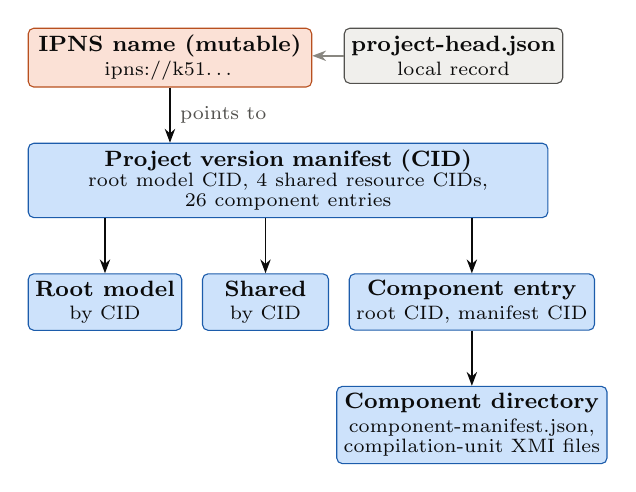
\begin{tikzpicture}[
  font=\footnotesize,
  >={Stealth[length=5pt]},
  box/.style={draw=inksoft, rounded corners=2pt, inner sep=2.5pt, align=center, text=ink, minimum height=7mm, anchor=north west},
  pointer/.style={box, fill=pointerfill, draw=pointerborder},
  immutable/.style={box, fill=immutablefill, draw=immutableborder},
  local/.style={box, fill=mutablefill},
  link/.style={->, draw=ink, line width=0.6pt},
  small/.style={font=\scriptsize, text=inksoft}
]

% Mutable head and the local record of the head
\node[pointer, minimum width=36mm] (ipns) at (0,0) {\textbf{IPNS name (mutable)}\\[-1pt]\scriptsize ipns://k51\ldots};
\node[local, minimum width=26mm] (head) at ($(ipns.north east)+(4mm,0)$) {\textbf{project-head.json}\\[-1pt]\scriptsize local record};
\draw[->, draw=muted, line width=0.6pt] (head.west) -- (head.west-|ipns.east);

% Project version manifest
\node[immutable, minimum width=66mm, text width=63mm] (manifest) at ($(ipns.south west)+(0,-7mm)$) {\textbf{Project version manifest (CID)}\\[-1pt]\scriptsize root model CID, 4 shared resource CIDs,\\[-2pt]\scriptsize 26 component entries};
\draw[link] (ipns.south) -- node[right, small] {points to} (ipns.south|-manifest.north);

% Entries of the manifest
\node[immutable, minimum width=16mm] (root) at ($(manifest.south west)+(0,-7mm)$) {\textbf{Root model}\\[-1pt]\scriptsize by CID};
\node[immutable, minimum width=16mm] (shared) at ($(root.north east)+(2.5mm,0)$) {\textbf{Shared}\\[-1pt]\scriptsize by CID};
\node[immutable, minimum width=29mm] (component) at ($(shared.north east)+(2.5mm,0)$) {\textbf{Component entry}\\[-1pt]\scriptsize root CID, manifest CID};
\foreach \target in {root, shared, component}
  \draw[link] (\target.north|-manifest.south) -- (\target.north);

% Content of one component
\node[immutable, minimum width=29mm, anchor=north] (dir) at ($(component.south)+(0,-7mm)$) {\textbf{Component directory}\\[-1pt]\scriptsize component-manifest.json,\\[-2pt]\scriptsize compilation-unit XMI files};
\draw[link] (component.south) -- (dir.north);

\end{tikzpicture}
\end{document}
